\chapter{Analisi di Copertura della Rete}
\label{cap:analisi}
Il simulatore ha permesso di ottenere i risultati riguardo la copertura dell'apparato \ac{LTE},
  
\section{Modellazione dello scenario}
\label{cap:dem}
In questa tesi è stato possibile simulare un modello tridimensionale degli ostacoli relativo ad una mappa esistente utilizzando 
la rappresentazione digitale delle quote di un territorio, usufruendo delle cosiddette mappe \ac{DTM}.
Sopra questo base è stato applicato un modello degli ostacoli, per generare uno scenario \emph{simile} a quello reale.
   
\subsection{Area di simulazione}
\label{sec:areasimu}
Per ottenere i dati relativi all'elevazione di una determinata area è stato necessario suddividere l'area come fosse una griglia, ogni
elemento della griglia è detto \emph{pixel}, in questa tesi ogni pixel ha le dimensioni di un quadrato di lato 5 m. \\
Successivamente è stato necessario assegnare ad ogni pixel la latitudine e la longitudine associata al centro di esso, ogni coordinata
dista quindi dalle adiacenti di circa 5 m.
L'area presa in considerazione è di circa $1 km \times 1 km$, quindi con una semplice divisione si ottiene che l'area, suddivisa in pixel, 
presa in esame equivale ad una matrice formata da $200 \times 200$ elementi, di cui ogni elemento contiene le coordinate esatte del centro 
del pixel. \\
È stato quindi sviluppato un semplice programma in \emph{Java} che permette la stampa su file di questi quarantamila elementi della 
matrice, elencati in colonna.

\subsection{Modello del terreno DTM}
Attraverso l'utilizzo del sito \url{http://www.gpsvisualizer.com/} è stato possibile importare la matrice output del programma citato 
nel paragrafo \ref{sec:areasimu} per ottenere l'elevazione di ogni coordinata.
Le elevazioni elencate nel file di output sono state rielaborate in una matrice con un altro programma in \emph{Java}, il risultato è 
quindi una matrice $200 \times 200$ contenente i dati dell'elevazione per ogni coordinata.
In Matlab è possibile effettuare un plot della matrice per rappresentare in tre dimensioni il modello del terreno come mostrato nella 
figura \ref{img:codem}.
\begin{figure}[h]
\centering
\caption{Modello tridimensionale del terreno della zona tra Colle Oppio e la stazione Roma Termini}
\label{img:codem}
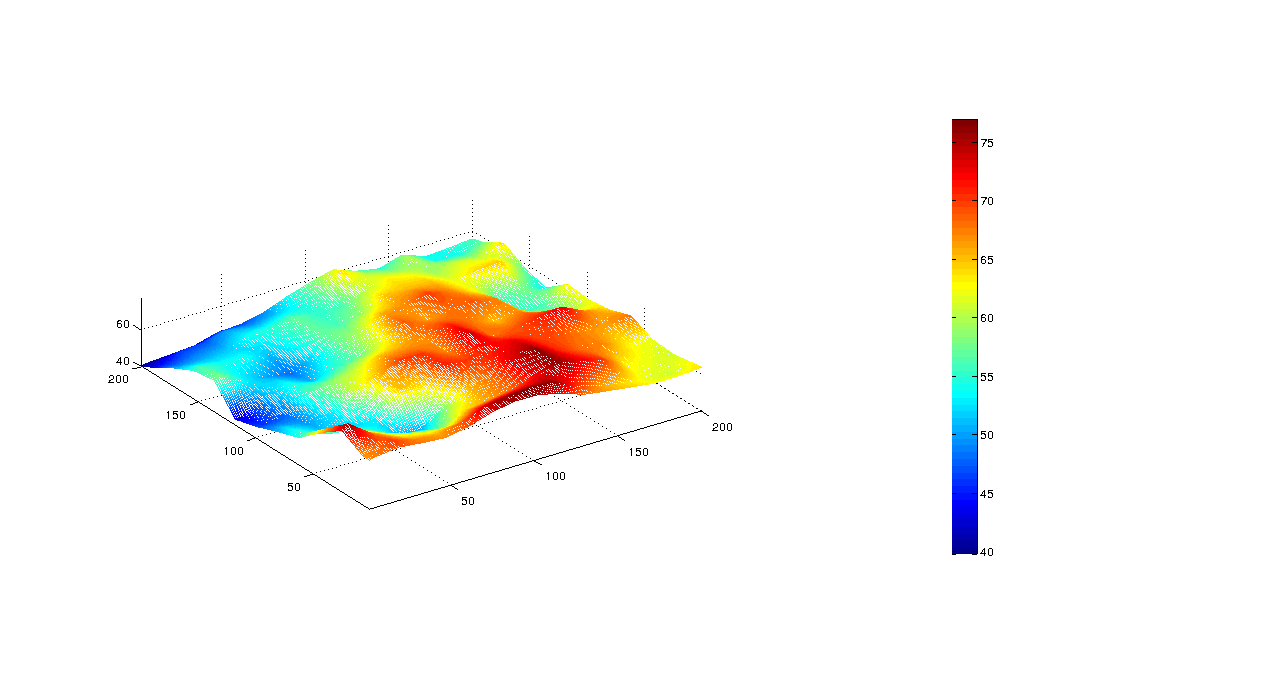
\includegraphics[scale=0.4]{Immagini/colleoppiodem}
\end{figure}

\subsection{Modello degli ostacoli}
Il processo che ha portato ad alla modellazione degli ostacoli è formato da più passi:
\begin{itemize}
\item Usufruendo delle \emph{API} di Google Maps è possibile fare una query http per ottenere la mappa dell'area interessata, in 
particolare per quanto riguarda l'area della zona tra Colle Oppio e la stazione Roma Termini è stato utilizzato l'url \\
\url{http://maps.google.com/maps/api/staticmap?center=41.895805,12.499113&zoom=15&size=1000x1000&sensor=false}
\begin{description}
\item \url{center=41.895805,12.499113} \\ indica le coordinate del centro della mappa statica.
\item \url{zoom=15} \\ indica il livello di zoom.
\item \url{size=1000x1000} \\ rappresenta la risoluzione dell'immagine.
\item \url{sensor=false} \\ in alcune applicazioni potrebbe essere necessario il sensore GPS per ottenere la posizione dell'utente, 
ma non è questo il caso
\item \url{&style=feature:all|element:labels|visibility:off} \\ infine aggiungendo questa stringa  al termine dell'url è possibile
togliere le etichette per visualizzare esclusivamente l'immagine della mappa.
\end{description}
il risultato è rappresentato nell'immagine successiva (\ref{img:comap}).
\begin{figure}[h]
\centering
\caption{Immagine statica della zona tra Colle Oppio e la stazione Roma Termini ottenuta tramite query http con Google Maps API.}
\label{img:comap}
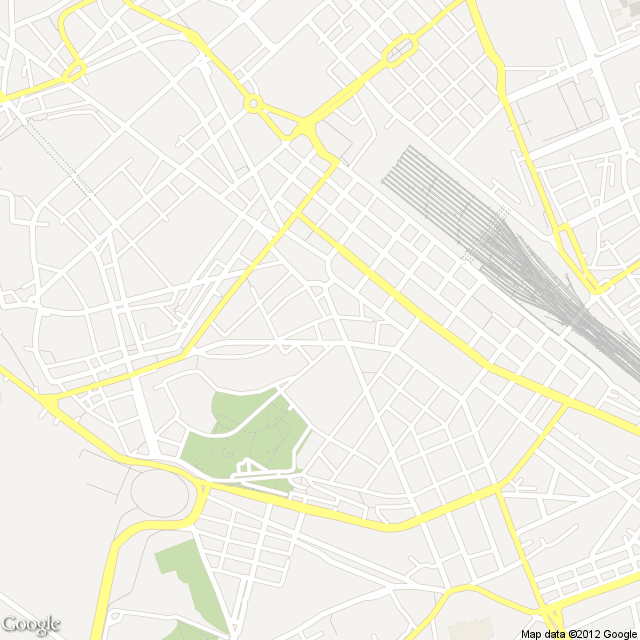
\includegraphics[scale=0.4]{Immagini/colleoppiomap}
\end{figure}
\item Il passo successivo è stato quello di rielaborare l'immagine per ottenere una maschera contenente gli ostacoli.
Per tale scopo è stato utilizzato \ac{GIMP}, software libero per la creazione e modifica di immagini digitali. \\
Per prima cosa è stata desaturata l'immagine, poi con l'aiuto di Google Earth è stato possibile evidenziare le aree piane e gli ostacoli;
è molto importante distinguere le due zone perché secondo i calcoli svolti in questa tesi, l'utente non può posizionarsi in 
corrispondenza degli ostacoli.
Avere quindi un modello degli ostacoli permette di verificare la copertura del sistema \ac{LTE} dell'\ac{UAV} in base alla posizione 
dell'utente. \\
Sono stati considerati come ostacoli costruzioni, monumenti e palazzi, quindi parchi, strade o, come in questo caso, la stazione in cui 
l'utente può sostare.
Gli ostacoli sono stati evidenziati in nero, tutto il resto è in bianco.
\begin{figure}[h]
\centering
\caption{Maschera degli ostacoli della zona tra Colle Oppio e la stazione Roma Termini ottenuta con \ac{GIMP} dalla mappa statica.}
\label{img:comask}
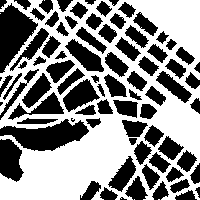
\includegraphics[scale=1]{Immagini/colleoppiomask}
\end{figure}

\subsection{Modello della mappa}
L'ultimo passo per arrivare ad un modello completo della mappa è stato quello di unire i due passaggi descritti nei due paragrafi
precedenti.
Il modello del terreno e la maschera degli ostacoli sono stati importati in Matlab, il risultato è quindi un modello tridimensionale
della mappa sul quale è applicata una maschera rappresentante la posizione di ogni ostacolo. \\
In Matlab è stato possibile sfruttare questo modello per ottenere una fedele rappresentazione tridimensionale dello scenario scelto. 
Sono stati utilizzati i dati dei modelli tridimensionali di \emph{Google Earth} come altezza, larghezza e lunghezza degli ostacoli, poi 
con l'aiuto di Matlab si è cercato di utilizzare questi dati per generare ostacoli con altezza, larghezza e lunghezza variabili nel
\emph{range} ottenuto da \emph{Google Earth}. \\
Il risultato è rappresentato nell'immagine sottostante. \\
\begin{figure}[!h]
\centering
\caption{Modello tridimensionale della zona tra Colle Oppio e la stazione Roma Termini.}
\label{img:modello}
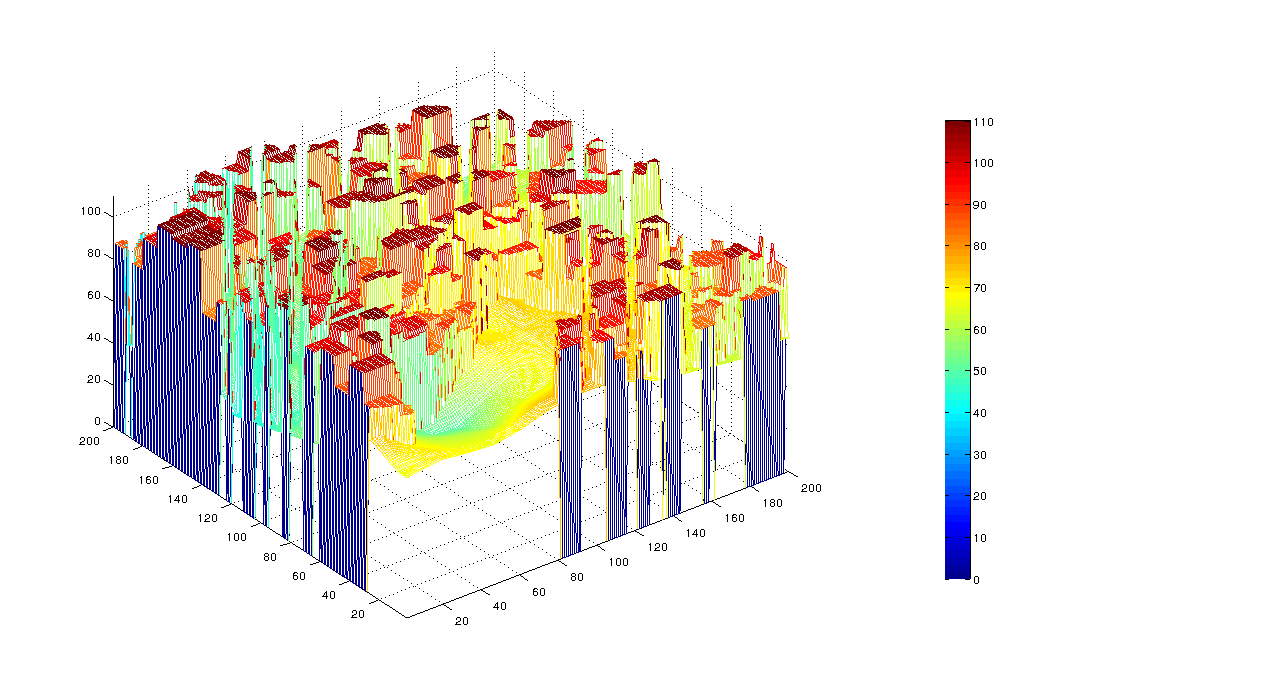
\includegraphics[scale=0.4]{Immagini/colleoppio}
\end{figure}
A questo punto è possibile utilizzare queste informazioni per modellare la copertura dell'apparato \ac{LTE} dell'\ac{UAV} su questo tipo 
di scenario.
\end{itemize}
\newpage
\section{Calcolo attenuazione}
Prima di descrivere come è stata calcolata l'attenuazione pixel $\times$ pixel è necessario richiamare alcuni concetti di propagazione
dell'onda elettromagnetica.

\subsection{Propagazione nello spazio libero}
Per propagazione nello spazio libero si intende una trasmissione del segnale elettromagnetico attraverso lo spazio libero o in mezzi 
tenui come l'atmosfera, in generale essa può suddividersi in radiopropagazione in un canale radio tra punti fissi (ponte radio) e 
radiopropagazione in un canale radiomobile tra terminali mobili e le stazioni radiobase. \\

\subsubsection{Attenuazione}
Un aspetto fondamentale di questo tipo di propagazione è l'attenuazione, questa può essere di due tipi:
\begin{description}
\item[attenuazione isotropica] è tipica dello spazio libero e la potenza diminuisce come $\frac{1}{d^{2}}$: \\
\[
p(d)=\frac{P_{T}}{4 \pi d^{2}}
\]
\item[attenuazione supplementare] si aggiunge a quella isotropica se il mezzo è diverso da quello vuoto.
\end{description}

\subsubsection{Fading} 
Nei collegamenti via etere all'ingresso del ricevitore il segnale giunge con improvvise e casuali variazioni di breve durata sia in 
ampiezza che in fase. Tali fluttuazioni sono note come fading o evanescenza. Il fenomeno è dovuto a varie cause.
Il \emph{fading per attenuazione} è dovuto alle variazioni fisiche dell'atmosfera che producono diverse attenuazioni del segnale in 
funzione della frequenza.
Il \emph{fading per interferenza} è dovuto all'interferenza tra i diversi segnali che partendo dal trasmettitore seguono molteplici 
percorsi prima di giungere al ricevitore. I segnali ricevuti hanno ampiezze e fase continuamente variabili poiché dipendono dallo 
stato fisico dell'atmosfera (pioggia, temporali, \ldots) dalla natura del suolo (mare, monti, \ldots) e dal cammino che le onde
elettromagnetiche seguono (onde dirette, onde riflesse dal suolo, \ldots).
I ricevitori sono dotati di opportuni sistemi di regolazione automatica atti a compensare ma non eliminare il fenomeno di fading.

\subsubsection{Diffrazione}
Il fenomeno della diffrazione permette la propagazione dei segnali radio sulla
superficie curva della Terra, oltre l'orizzonte e oltre 
i vari ostacoli che può incontrare. Anche nel caso in cui la potenza del segnale ricevuto decresce rapidamente quando il trasmettitore 
si muove all'interno di regioni così dette in ombra, il segnale generato dalla diffrazione è sufficientemente potente da produrre un 
segnale utile. \\
La diffrazione può essere spiegata mediante il principio di Huygen, che afferma che tutti i punti appartenenti ad un fronte d'onda 
possono essere considerati come sorgenti di nuove onde; tali onde si combinano per produrre un
nuovo fronte che si propaga nella 
stessa direzione del primo; è questo secondo
fronte d’onda che permette la propagazione del segnale nelle regioni in ombra. \\

\subsubsection*{Zone di Fresnel}
Mediante le zone di Fresnel è possibile caratterizzare l'attenuazione dovuta a diffrazione in relazione alla differenza di cammino 
che le onde
devono compiere per aggirare un ostacolo posto tra trasmettitore e ricevitore.
Le zone di Fresnel rappresentano regioni successive in cui le onde secondarie
devono percorrere, per raggiungere il ricevitore 
dal trasmettitore, una distanza
maggiore di $n\frac{\lambda}{2}$ rispetto al cammino lungo la \ac{LOS}.
\begin{figure}[h]
\centering
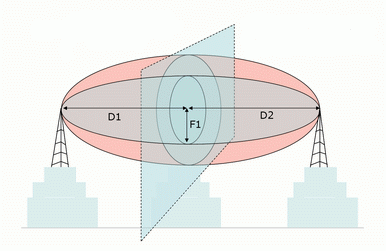
\includegraphics[height=0.5\textwidth]{Immagini/fresnel}
\caption{I confini delle zone di Fresnel costituiti da cerchi concentrici nel caso in cui tra le due antenne non sono presenti ostacoli.}
\label{img:fresnel}
\end{figure}
La differenza tra il cammino diretto e il cammino rifratto che attraversa ogni cerchio è $n\frac{\lambda}{2}$, i raggi dei cerchi che 
delimitano le zone di Fresnel dipendono dal punto in cui è posto il piano, così le zone avranno raggio massimo nel punto centrale tra 
i due dispositivi e tali raggi andranno a rimpicciolirsi se il piano è mosso tra trasmettitore e ricevitore. \\

\subsubsection*{Ostacolo singolo: modello a lama di coltello}
La stima dell’attenuazione del segnale causato da diffrazione per onde radio in un ambiente non ottimale, in presenza per esempio di 
costruzioni o colline, come modellato in questa tesi, è solitamente difficile da effettuare con precisione. Quando la zona d'ombra in 
cui si viene a trovare il dispositivo ricevitore è generata da un unico oggetto che si frappone tra ricevitore e trasmettitore, 
l'attenuazione causata dalla diffrazione può essere stimata considerando l'ostacolo come un piano il cui spessore è minimo. \\
Questo è il più semplice modello di diffrazione in cui l'attenuazione del segnale causata da un tale fenomeno viene messa in relazione 
con quanto l'ostacolo invade la prima zona di Fresnel: più l'ostacolo entra nella prima zona di Fresnel e più il segnale arriva al 
ricevitore attenuato. \\
Il campo elettrico ricevuto ha una precisa soluzione analitica:
\begin{align}
\mathbf{E}_{d} = \mathbf{E}_{0} I(v) = \mathbf{E}_{0} \frac{1+j}{2} \int_{2}^{\infty} e^{-j \frac{2 \pi}{2} t^{2}}\, dt
\label{eq:ed}
\end{align}
dove $\mathbf{E}_{d}$ è il campo elettrico ricevuto, $\mathbf{E}_{0}$ è il campo elettrico che si avrebbe nello spazio libero e $v$ è
il \emph{parametro di diffrazione di Fresnel-Kirkhoff}, pari a:
\begin{align*}
 \label{eq:parametrodiffrazione}
 v = h \sqrt{\frac{2(d_{1} + d_{2})}{\lambda d_{1} d_{2}}}
\end{align*}
dove
\begin{description}
\item $h$ è la distanza tra la congiungente tre le antenne e l'estremità dell'ostacolo, la distanza $h'$ nella figura \ref{img:knifeedge}
è detta \emph{franco}.
\item $d_{1}$, $d_{2}$ sono, rispettivamente, le distanze tra trasmettitore ed ostacolo e tra ostacolo e ricevitore.
\item $\lambda$ è la lunghezza d'onda, $\lambda = \frac{c}{f}$
\end{description}
\begin{figure}[!h]
\centering
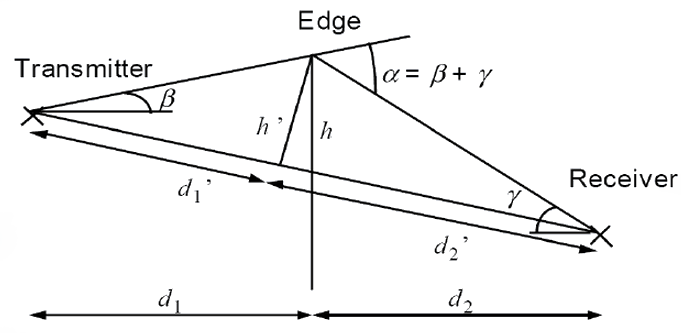
\includegraphics[height=0.5\textwidth]{Immagini/knifeedge}
\caption{Nell'origine l'ostacolo a lama di coltello con altezza h.}
\label{img:knifeedge}
\end{figure}
La funzione del parametro di diffrazione nell'equazione \ref{eq:ed} è l'integrale complesso di \emph{Fresnel}:
\begin{align}
\label{eq:integralefresnel}
I(v) = C(v) - jS(v)
\end{align}
con
\begin{align*}
 C(v)=\int_{0}^{v} \cos(\frac{\pi}{2}u^{2})\, du \\
 S(v)=\int_{0}^{v} \sin(\frac{\pi}{2}u^{2})\, du \\
\end{align*}
Le funzioni $C(v)$ e $S(v)$ sono dette, rispettivamente, integralcoseno e integralseno, il loro andamento, uno in funzione dell'altro,
è rappresentato nella figura \ref{img:cornu}, nella cosiddetta spirale di \emph{Cornu}:
\begin{figure}[!h]
\centering
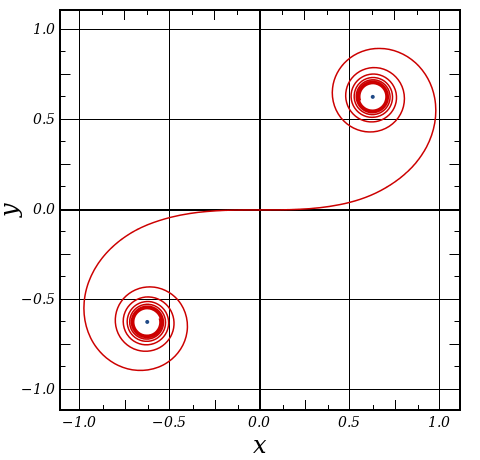
\includegraphics[height=0.5\textwidth]{Immagini/cornu}
\caption{Spirale di Cornu.}
\label{img:cornu}
\end{figure}
Dai valori asintotici $C(\infty) = S(\infty) = 0.5$ e $C(-\infty) = S(-\infty) = -0.5$, si ottiene, sostituendo nella (\ref{eq:ed}):
\[
\mathbf{E}_{d} = \mathbf{E}_{0} \frac{1+j}{2} 
\left \{ \left [ \frac{1}{2} - C(v) \right ] + j \left [ \frac{1}{2} - S(v) \right ] \right \}
\]
dalla quale si ottiene la \emph{perdita supplementare per diffrazione}:
\[
 L_{D}(dB) = -20 \log{F_{D}}
\]
Si definisce fattore di diffrazione, $F_{d}$, il rapporto tra l'ampiezza del campo ricevuto e quella nello spazio libero:
\begin{align*}
F_{d} \doteq& \left| \frac{\mathbf{E}_{d}}{\mathbf{E}_{0}}  \right| = \\
=& \frac{\sqrt{2}}{2} \left| \frac{1}{2} (1-j) - I(v) \right| = \\
=& \frac{\sqrt{2}}{2} \sqrt{ \left [ \frac{1}{2} - C(v) \right ]^{2} + \left [ \frac{1}{2} - S(v) \right ]^{2} }
\end{align*}
Nella figura \ref{img:fd} è rappresentato l'andamento di $F_{d}$ in funzione del parametro di diffrazione $v$. \\
\begin{figure}[!h]
\centering
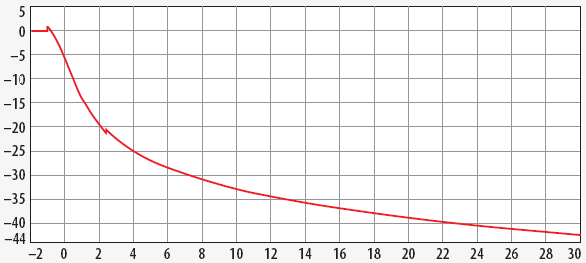
\includegraphics[height=0.5\textwidth]{Immagini/pathloss}
\caption{Andamento del fattore di diffrazione in funzione del parametro di diffrazione.}
\label{img:fd}
\end{figure}
Visivamente l'attenuazione per ostacolo singolo è ben descritta nella figura \ref{img:knifeedgeeffect}, il segnale trasmesso incide 
l'ostacolo, il quale diventa poi nuova sorgente e permette il passaggio del segnale al ricevitore, l'altezza dell'ostacolo può anche 
essere superiore a quella dell'apparato trasmittente o ricevitore.
\begin{figure}[!h]
\centering
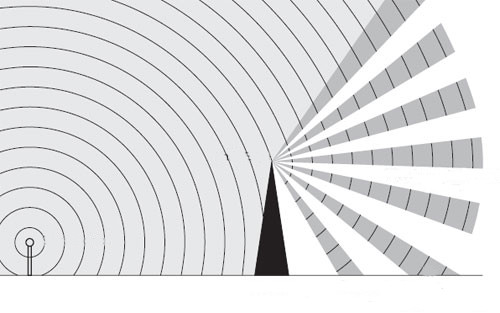
\includegraphics[height=0.5\textwidth]{Immagini/knifeedgeeffect}
\caption{Il segnale si propaga fino all'ostacolo che poi diventa la nuova sorgente.}
\label{img:knifeedgeeffect}
\end{figure}

\subsubsection*{Ostacolo multiplo: Metodo di Epstein-Peterson}
\label{sec:epsteinpeterson}
Nel caso di più ostacoli che si interpongono tra trasmettitore e ricevitore, è spesso utilizzato il modello di Epstein-Peterson.
Secondo questo modello la distanza tra trasmettitore e ricevitore può essere suddivisa in parti differenti, come mostrato in figura
\ref{img:epsteinpeterson} la perdita dovuta alla diffrazione sarà calcolata in base a queste parti. Si procede seguendo più passi:
\begin{itemize}
\item  l'attenuazione dovuta alla lama di coltello in Q1 si calcola considerando l'altezza dell'ostruzione relativa alla linea che 
congiunge l'antenna emittente con l'estremità dell'ostruzione in Q2, come se vi fosse collocata l'antenna ricevente. Il parametro 
di diffrazione di Fresnel-Kirkhoff, $v$, fornisce:
\[
v(Q1) = (d_{1},d_{2},h_{1}-h_{2}\frac{d_{1}}{d_{1}+d_{2}})
\]
si ricava quindi $F_{D}(v_{Q1})$
\item l'attenuazione dovuta alla lama di coltello in Q2 si calcola considerando l'altezza dell'ostruzione relativa alla linea, come 
se in B fosse collocata l'antenna emittente, il parametro $v$ sarà pari a:
\[
v(Q2) = (d_{2},d_{3},h_{2}-h_{1}-(-h_{2})\frac{d_{2}}{d_{2}+d_{3}})
\]
si ricava quindi $F_{D}(v_{Q2})$
\end{itemize}
L'attenuazione per diffrazione dovuta al contributo dei due ostacoli è pari alla somma (in $dB$) delle due attenuazioni appena calcolate:
\[
L_{D} = -10 \log F_{D}(v_{Q1}) - 10 \log F_{D}(v_{Q2})
\]
Al crescere della distanza tra gli ostacoli, applicando il metodo di \emph{Epstein-Peterson}, si ottengono risultati sempre più accurati.
Per ostacoli molto vicini, invece, questo tipo di metodo potrebbe non essere molto accurato.
\begin{figure}[h]
\centering
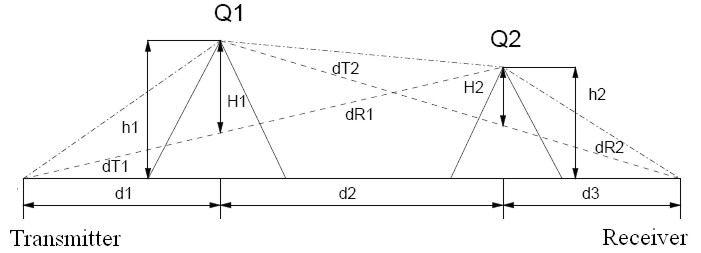
\includegraphics[height=0.3\textwidth]{Immagini/epsteinpeterson}
\caption{Il segnale si propaga fino all'ostacolo successivo che poi diventa la nuova sorgente, così fino al dispositivo ricevitore.}
\label{img:epsteinpeterson}
\end{figure}

\subsubsection{Bilancio di radiocollegamento}
\label{cap:bilancio}
Per bilancio di radiocollegamento, in inglese \emph{Link Budget}, si intende l'insieme dei guadagni e delle perdite dall'apparato
trasmettitore, attraverso il mezzo (spazio libero, cavo, fibra, \ldots), fino all'apparato ricevitore, in un sistema di telecomunicazioni. \\
Essa rappresenta l'attenuazione dovuta alla propagazione del segnale trasmesso, così come i guadagni di antenna le perdite di linea o 
di altra natura.
I guadagni di canale casualmente variabili come il fading sono presi in considerazione aggiungendo qualche margine a seconda della gravità 
prevista dei suoi effetti.
\\[1cm]
Un semplice esempio di equazione di bilancio di radiocollegamento è come questa:
\begin{align*}
Potenza Ricevuta [dBm] &= Potenza Trasmessa [dBm] &+ \\
&+ Guadagni [dB] &+ \\
&- Perdite [dB]
\end{align*}

Per sistemi \ac{LOS} la prima causa di perdita è la diminuzione della potenza del segnale dovuta alla propagazione uniforme, proporzionale
al quadrato inverso della distanza. Nel calcolo della potenza ricevuta si devono considerare alcuni fattori e semplificazioni che rendono
il calcolo più agevole:
\begin{itemize}
\item Le antenne trasmittenti sono per la maggior parte non isotropiche.
\item Antenne omnidirezionali sono molto rare nelle telecomunicazioni, quindi in ogni equazione di bilancio di radiocollegamento si deve
considerare il guadagno di antenna.
\item  Le antenne trasmittenti concentrano la potenza del segnale nella direzione in cui sono rivolte le antenne riceventi.
\item Il termine della lunghezza d'onda è spesso considerato parte dell'equazione della perdita nello spazio libero. 
Questa riduzione di complessità è accettabile per sistemi di comunicazione terrestri, considerando percorsi \ac{LOS}.
\item Si considera la propagazione dell'onda portante indipendente dalla lunghezza d'onda, questo è giustificato legge della 
conservazione dell'energia, la quale richiede che il campo elettrico diminuisca in potenza come il quadrato della distanza 
indipendentemente dalla frequenza (nello spazio libero).
\item Il cablaggio tra le radio e le antenne può introdurre significative perdite supplementari.
\item Effetto doppler induce perdita di potenza nel ricevitore. 
\end{itemize}
\subsubsection{Equazione}
\[
 P_{Rx} = P_{Tx} + G_{Tx} - L_{Tx} - L_{FS} - L_{M} + G_{Rx} - L_{Rx}
\]
dove \\
$P_{Rx}$ è la potenza ricevuta \\
$P_{Tx}$ è la potenza trasmessa \\
$G_{Tx}$ è il guadagno dell'antenna \\
$L_{Tx}$ sono le perdite del trasmettitore \\
$L_{FS}$ è la perdita nello spazio libero \\
$L_{M}$ indica perdite varie (margine di fading, polarizzazione non corrispondente, \ldots) \\
$G_{Rx}$ è il guadagno dell'antenna ricevente \\
$L_{Rx}$ sono le perdite del ricevitore \\

\subsubsection{Margine di radiocollegamento}
Per compensare il fenomeno del fading si cerca di aumentare il livello di potenza del segnale in uscita di una quantità detta
\emph{margine di fading $M_{F}$} in modo da mantenere per tutta la durata del collegamento un sufficiente \ac{SNR}. \\
Il valore di $M_{F}$ necessario a garantire una prefissata affidabilità del collegamento è valutato in base ad analisi teoriche e 
sperimentali. Per esempio per comunicazioni satellitari, che operano a $10GHz$ è sufficiente un margine di fading $M_{F} = 6 dB$. \\
Per i collegamenti in ponte radio terrestri si suppone che il fading segua una \emph{distribuzione di Rayleigh}, si definisce la 
disponibilità del collegamento come:
\[
 D = e^{-\frac{P_{min}}{P_{R}}}
\]
dove $P_{min}$ è la potenza minima che il ricevitore è in grado di riconoscere e $P_{R}$ è la potenza effettivamente ricevuta, il margine
di fading si ottiene quindi dalla relazione:
\[
 (M_{F})_{dB} = -10\log{\left | \ln{D} \right | }
\]

\begin{table}[h]\footnotesize
\caption{Valori caratteristici del margine di radiocollegamento.}
\label{tab:margine}
\begin{tabularx}{\textwidth}{XX}
\toprule
Disponibilità D del collegamento (\%) & Margine di fading $M_{F}$ (dB) \\
\midrule
90 & 10 \\
99 & 20 \\
99.9 & 30 \\
99.99 & 40 \\
99.999 & 50 \\
\bottomrule
\end{tabularx}
\end{table}

Nel caso considerato, la somma tra $P_{Tx}$, $G_{Tx}$ e perdita dei cavi è detta \ac{EIRP} ed è pari a circa $62 dBm$. Si considera, inoltre,
la \emph{sensitività del ricevitore}, la quale è data dalla somma tra cifra di rumore, rumore termico e \ac{SINR}, la somma di questi
tre fattori è circa $106.4 dBm$. \\
Infine è aggiunto il margine di interferenza, il guadagno dell'antenna ricevente $G_{Rx}$ e il controllo di canale. \\
Nel simulatore è stata fatta variare la potenza trasmessa per prolungare la durata della batteria del velivolo, l'attenuazione massima 
in grado di riconoscere il ricevitore è di $163.5 dBm$ per potenza trasmessa di $46 dBm$, $141.5 dBm$ per $24 dBm$ trasmessi e $137.5 dBm$
per $20 dBm$ trasmessi.

\section{Analisi di Copertura della Rete}
\label{cap:copertura}
Una volta modellato il terreno e gli ostacoli come descritto nel capitolo \ref{cap:dem}, si è cercato di analizzare la copertura 
del sistema \ac{LTE} montata sull'\ac{UAV}.

\subsection{Calcolo dell'area coperta}
L'attenuazione è stata calcolata in ogni pixel valido della mappa, per pixel valido si intende qualsiasi pixel che non rappresenti un 
ostacolo. \\
Per ottenere l'attenuazione è stato sviluppato un script Matlab interagente con quello descritto nel capitolo \ref{cap:dem}, questo 
programma riceve in \emph{input} i dati della mappa come altezze del terreno, posizione e altezza degli ostacoli e le coordinate e l'altezza
dell'\ac{UAV}. Una volta lanciato lo script si otterranno tre matrici delle stesse dimensioni della mappa:
\begin{itemize}
\item La prima restituisce l'attenuazione \emph{free space} pixel $\times$ pixel.
\item La seconda contiene l'attenuazione \emph{supplementare} dovuta alla presenza di ostacoli.
\item La terza è la somma delle prime due e rappresenta l'attenuazione totale pixel $\times$ pixel.
\end{itemize}

\subsubsection{Ostacoli tra elicottero ed utente}
L'individuazione di tutti gli ostacoli che si frappongono tra elicottero ed utente, su una linea retta, permette di calcolare la 
diffrazione del segnale in modo da poter applicare quanto visto nel paragrafo \ref{sec:epsteinpeterson}. \\
Questo tipo di problema si traduce nell'applicazione di concetti di base di geometria. Per prima cosa è stato suddiviso lo spazio in 
due aree individuate dal valore del coefficiente angolare della retta passante per elicottero ed utente: come mostrato nella figura
\ref{img:areagriglia} nelle zone in celeste il coefficiente angolare della retta passante per due punti varia tra -1 e +1 altrimenti la 
retta passa per la zona arancione. Il sistema di riferimento è centrato sulle coordinate dell'elicottero.
\begin{figure}[h]
\centering
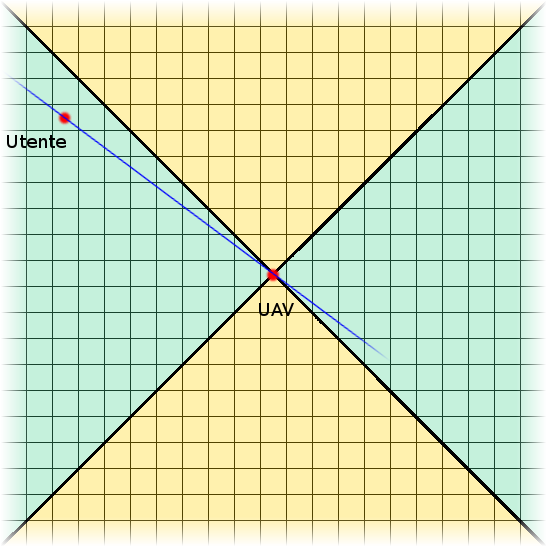
\includegraphics[height=0.7\textwidth]{Immagini/areagriglia}
\caption{Suddivisione dell'area da analizzare.}
\label{img:areagriglia}
\end{figure}
Per individuare gli ostacoli che incontrano la retta è stato campionato l'asse delle ascisse, o delle ordinate a seconda della zona, in
modo da controllare tutti i punti intermedi tra un pixel e l'altro. Come $x$ si prende una lista di valori che va dalla $x_{e}$, ascissa
dell'elicottero, fino alla $x_{u}$, ascissa dell'utente. Da questa lista di coordinate è facile ottenere i rispettivi valori delle 
ordinate:
\begin{equation}
\textbf{y} = y_{u} + \frac{y_{e}-y_{u}}{x_{e}-x_{u}}(\textbf{x}-x_{u})
\label{eq:rettaduepunti}
\end{equation}
dove $\textbf{x}$ e $\textbf{y}$ sono vettori contenenti la lista di coordinate. \\
La suddivisione in zone è molto importante, se si campionasse solo lungo l'asse delle ascisse, per rette quasi verticali si avrebbero 
pochi valori da controllare, così invece, è possibile campionare le rette sfruttando tutta la loro lunghezza. \\
Con questo tipo di approccio si evidenzierà una zona limitrofa alla retta (regione in giallino), dove sarà necessario controllare la 
presenza degli ostacoli:
\begin{figure}[h]
\centering
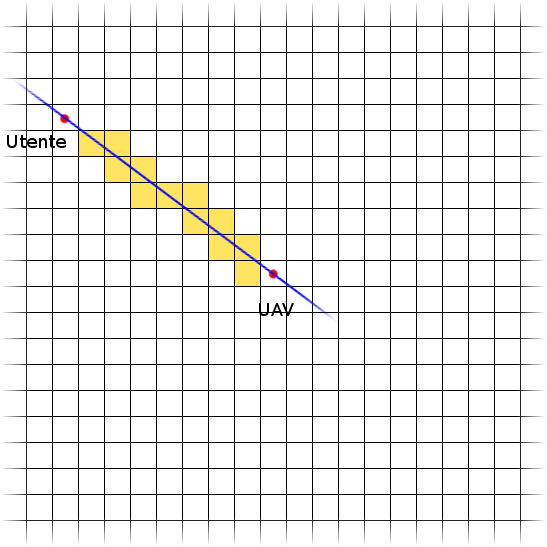
\includegraphics[height=0.7\textwidth]{Immagini/quadretti}
\caption{Pixel passanti per la retta.}
\label{img:quadretti}
\end{figure}
Ottenute tutti i pixel per cui passa la retta, si deve prendere la parte intera di ogni coordinata per ottenere il pixel 
corrispondente; a questo punto si deve controllare se ogni pixel faccia parte di un ostacolo: si prende la maschera degli ostacoli 
(\ref{img:comask}) e si controlla se il pixel appartenga o meno all'ostacolo. \\
Evidenziati gli ostacoli dall'area in giallino della figura \ref{img:quadretti} è necessario distinguere gli ostacoli in base alla loro
altezza; il modello di Epstein-Peterson, infatti, permette di modellare un ostacolo come se fosse una lama di coltello, quindi se più
pixel vicini hanno la stessa altezza faranno parte dello stesso ostacolo e nella lista degli ostacoli tra elicottero ed utente dovranno
essere considerati come uno solo.
Il modello di Epstein-Peterson sulla diffrazione dovuta ad ostacoli multipli è definito su una retta, l'area in giallino, invece, definisce
una zona limitrofa alla retta tra elicottero ed utente: si devono quindi proiettare le coordinate degli ostacoli sulla retta. \\
Per implementare ed automatizzare la proiezione del pixel sulla retta sono stati utilizzati dei semplici concetti di geometria analitica;
dati tre punti, coordinate dell'elicottero, coordinate dell'utente e coordinate dell'ostacolo si devono calcolare le coordinate della 
proiezione in funzione di questi tre punti:
\begin{align*}
E &= (x_{e},y_{e}) \\
U &= (x_{u},y_{u}) \\
O &= (x_{o},y_{o}) \\
\end{align*}
Si considera la retta (\ref{eq:rettaduepunti}) passante per $E$ ed $U$, la perpendicolare passante per $O$ avrà equazione:
\begin{equation}
y = y_{o} - \frac{x_{e}-x_{u}}{y_{e}-y_{u}}(x-x_{o})
\label{eq:perpendicolareost}
\end{equation}
L'intersezione della retta \ref{eq:rettaduepunti} con la \ref{eq:perpendicolareost}, mi darà le coordinate della proiezione dell'ostacolo
sulla retta, i punti in verde nell'immagine \ref{img:proiezioni}.
\begin{align*}
x &= \frac{(y_{o}-y_{e}) (y_{u}-y_{e}) (x_{u}-x_{e}) + x_{o} (x_{u}-x_{e})^{2} + x_{e} (y_{u}-y_{e})^{2}}
	  {(y_{u}-y_{e})^{2} + (x_{u}-x_{e})^{2}} \\
y &= y_{e} + (y_{u}-y_{e}) \frac{(y_{o}-y_{e}) (y_{u}-y_{e}) + (x_{o}-x_{e}) (x_{u}-x_{e})}
			        {(y_{u}-y_{e})^{2} + (x_{u}-x_{e})^{2}}
\end{align*}
\begin{figure}[h]
\centering
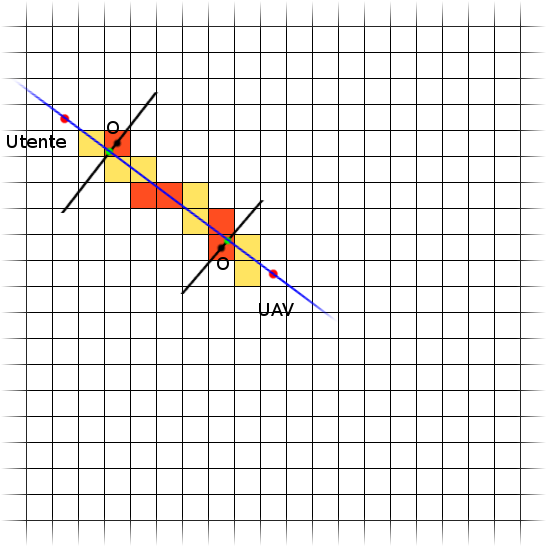
\includegraphics[height=0.7\textwidth]{Immagini/proiezioni}
\caption{Proiezioni degli ostacoli sulla retta.}
\label{img:proiezioni}
\end{figure}
Dopo aver calcolato la proiezione di ogni ostacolo sulla retta si ottiene una lista di ostacoli tra elicottero ed utente, adesso è possibile
applicare il modello di Epstein-Peterson per calcolare l'attenuazione dovuta alla diffrazione.

\subsubsection{Parametro di diffrazione}
Il modello di Epstein-Peterson si riduce a calcolare l'attenuazione dovuta ad un singolo ostacolo ed a replicare il calcolo ostacolo per 
ostacolo, Quindi il problema del calcolo della diffrazione per ostacolo multiplo può essere semplificato al calcolo per ostacolo singolo. \\
Partendo quindi dalla lista di ostacoli tra elicottero ed utente si calcola la distanza tra elicottero e primo ostacolo e tra ostacolo 
ed utente, infine si calcola il franco e si applica la formula \ref{eq:parametrodiffrazione} per ottenere il \emph{parametro di diffrazione}.

\subsubsection{Attenuazione dovuta alla diffrazione}
Il calcolo dell'attenuazione pixel $\times$ pixel è quasi terminato, adesso si ha per ogni pixel il parametro di diffrazione dovuto agli
ostacoli che si frappongono tra elicottero ed utente. \\
Il parametro di diffrazione permette di calcolare le due funzioni integralcoseno ed integralseno, le quali sottratte tra loro restituiscono
l'integrale complesso di Fresnel (\ref{eq:integralefresnel}).
Quest'ultimo valore permette di ottenere il fattore di diffrazione $v$, il quale, calcolato in dB, dà l'attenuazione nel determinato
pixel. \\
Ripetendo il processo per ogni pixel della matrice, si otterranno le matrici con l'attenuazione (free space, supplementare e totale)
calcolata per ogni pixel.


\subsubsection{Calcolo del raggio di copertura}
Il calcolo del raggio di copertura permette di evidenziare l'area coperta dal segnale trasmesso dall'\ac{UAV}, in base all'attenuazione
massima tollerabile dal ricevitore. \\
Per il calcolo dell'attenuazione è stata seguita la procedura descritta nel capitolo \ref{cap:bilancio}, una volta ottenuta questa soglia
si procede a confrontarla con l'attenuazione calcolata in ogni pixel, se quest'ultima è superiore allora si suppone che quel pixel non
sia coperto dal segnale trasmesso dall'\ac{UAV}.
A questo punto il calcolo del raggio si semplifica in una semplice distanza tra due punti:
\begin{figure}[h]
\centering
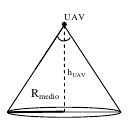
\includegraphics[height=0.3\textwidth]{Immagini/raggio}
\caption{Il raggio è la distanza sul piano tra \ac{UAV} ed utente coperto da segnale.}
\label{img:raggio}
\end{figure}
Il raggio viene quindi calcolato per ogni punto coperto, il risultato è una matrice contenente le distanze tra elicottero ed utente. \\

Una volta calcolato il raggio di copertura pixel $\times$ pixel è possibile calcolare il raggio medio di copertura come la media 
aritmetica tra i raggi ottenuti, così facendo si otterrà un'area circolare dove la maggior parte del segnale sarà concentrato. \\
Oltre al raggio medio di copertura, un indice più veritiero della copertura totale del segnale è dato dai percentili del raggio di 
copertura; presi tutti i raggi punto per punto è stato calcolato l'$80^o$ percentile in modo da rappresentare il raggio che contiene 
l'$80\%$ dell'area coperta da segnale.

\subsubsection{Miglioramento di copertura dell'area}
Al fine di migliorare i settori esclusi dai calcoli precedenti, dove l'attenuazione del segnale è superiore alla massima consentita, sarà
possibile proseguire secondo due approcci: la variazione della posizione degli \ac{UAV} e l'utilizzo di più \ac{UAV}.
La prima possibilità prevede di far seguire ad un \ac{UAV} un loop sull'area da coprire, in modo da offrire, anche se per una durata 
limitata, ad ogni utente il segnale per poter comunicare nell'area. \\
Con la seconda possibilità si coordineranno più \ac{UAV} a formare una rete a maglie, la cosiddetta rete \emph{mesh}, in modo da poter
coprire un'area molto più estesa. \\ 
Le due possibilità, ovviamente, potrebbero anche coesistere a seconda delle esigenze dei soccorritori, come per esempio per l'espansione
dell'area, il numero di \ac{UAV} a disposizione, \ldots